\chapter{Model}
  The model is the most important part of the project. An invalid model can only hope to produce an invalid simulation. This chapter will describe the model used during this project, comparing it with the real world and attempting to note and justify any simplifications or assumptions used. The first section gives an overview of the model. The following sections then looks at specific parts in more detail.
  
  \section{Overview}
    The aim of modelling is to highlight which the features in the environment to be simulated are important and which can be ignored\cite{Sterling2009}. For an agent-based model we wish to break these features down into the agents and their environment and their interactions with that environment so that the agents may assess their situation and make decisions\cite{Bonabeau2002}. In this section there is a quick summary of the important features of the model and their relationships.
    
    The agents in this model are coxes. The main features of their environment are the boat in which they sit and those in containing other coxes and the river on which these boats sit. The coxes interacts with the environment through actions which will determine how the boat behaves, with the cox aiming to safely navigate the boat from one end of the river to the other. It should also be noted that at one end of the river sits a Boat House from which new boats are launched and to which a cox must return its boat and land.
    
    The model is cox-centric. For instance, the model does not aim to replicate how the rowers in a boat implement a cox's orders. However, the best way to describe the model is to work from the bottom up spatially. At the bottom there is the river. This is the entity shared by all boats and defines the positional constraints placed upon them. Every boat must be fully on the river. The river is made up of 3 lanes which can be thought of as 1 dimensional spaces broken up by regular marker nodes, in other words a graph where each node represents a particular point on the river and each edge represents a connection to the next point in the lane either upstream or downstream (so each node only has one edge in and one edge out). By mapping each node's location to a 2 dimensional space and assuming that there is a channel of water about 10 metres wide between each connected node, the river can then be drawn as the union of these lanes.
    
    In the middle is the boat. The boat can be considered as the embodiment of the cox. It is the boats that sit on the river and should not be allowed to overlap with the bank or another boat. When the cox carries out an action it is by altering properties of the boat such as it's speed and direction. No attempt has been made to model directly the rowers who in reality do the hard work of actually propelling the boat along the river. At each tick of the clock the boat will move based on the current value of its properties, which may have just been altered by the cox. It should be noted that outside forces other than the cox can act on the boat. For instance, should two boats try and travel along the same edge in a lane then they will crash and come to a complete standstill for a while.
    
    At the top, sits the cox. The cox can make observations about the state of its own boat and the river nearby (should the boat be travelling faster? are there any nearby boats? is the boat nearing the end of river?). At each tick of the clock the cox uses these observations to decide which action to perform next and then executes it. It should be noted the actions themselves will may then behaviour differently depending on the boat's situation, for example, a boat at its maximum speed will not change speed even if the cox decides to execute the Speed Up action.
    
    One final feature that is worth mentioning and sits slightly apart from the cox-boat-river layered view of the model is the Boat House. It might itself be considered an agent since it autonomously launches boats, but as neither launching nor landing can be considered intelligent processes from the Boat House's point of view for the purposes of describing the model it fits more naturally as part of a part of the river since it also marks one end of the river beyond which a boat cannot pass.
    
    Figure \ref{fig:modeloverview} provides a summary the relations between the 4 main features of the model just described. The following sections will then describe in more detail the river, the boats and the coxes and their decision making processes.
    
    \begin{figure}[H]
    \begin{center}
    	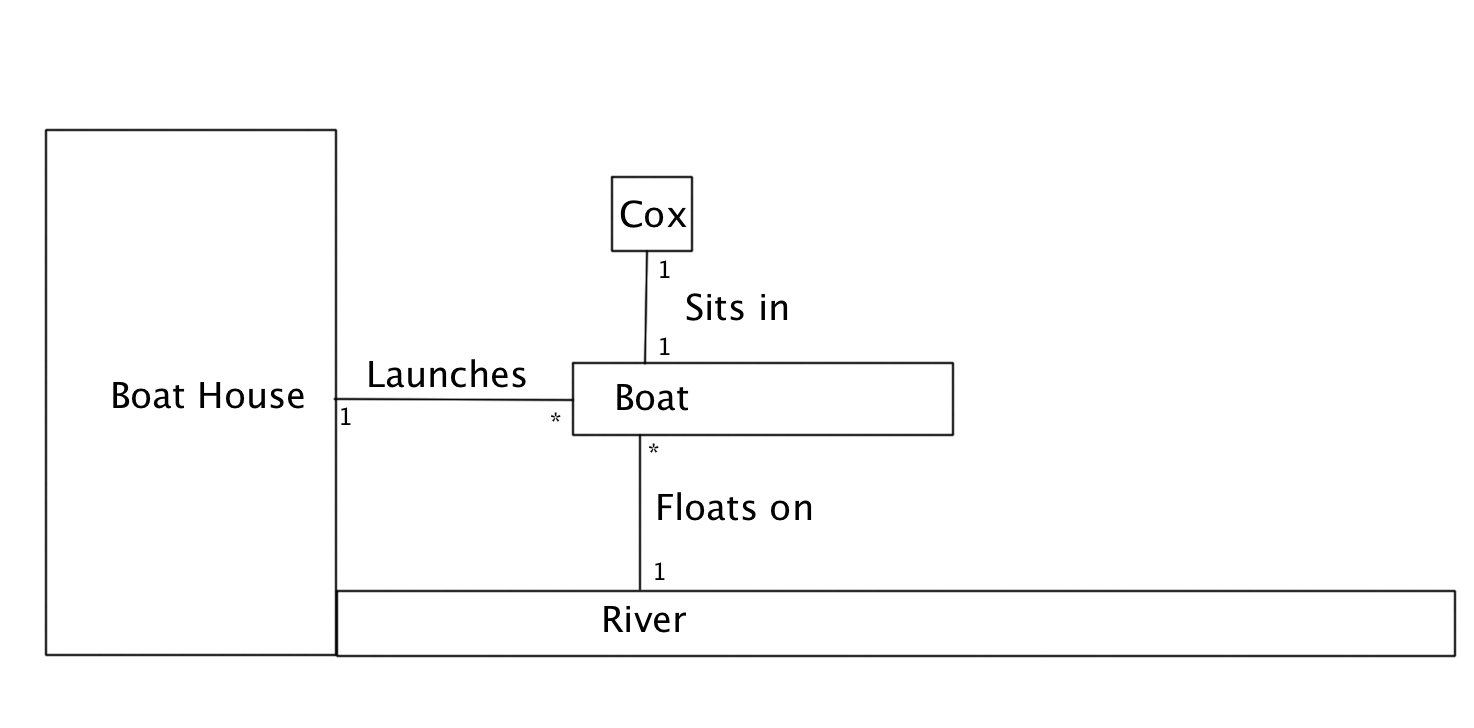
\includegraphics[scale=0.3]{images/ModelOverview.png}
    	\caption{Model Overview}
    	\label{fig:modeloverview}
    \end{center}
    \end{figure}

    \section{River}
      \paragraph{Physical description}
      Most rowing on the Cam takes places in the 5km between Jesus Lock and Baits Bite Lock. A few crews sometimes carry their boats over Baits Bite Lock to another stretch of river up to Bottisham lock. The boathouses used by rowers are clustered near Jesus Lock. The first 2km from Jesus Lock are quite narrow and windy. This section is used for warm-ups and warm-downs and in theory on this part of the river crews are not supposed to row at full pressure. It is in the 3km about to Baits Bite lock that the most varied rowing takes place. The river has been known to flood but for the most part it is static and its stream has no effect on boats. The river bank is varied and there are many landmarks such as corners, bridges, trees, and buildings by the river. The width of the river varies between wide enough to allow 3 crews to be side-by-side down to a bottleneck where only one crew can pass at a time.
      
      \subsection{Simplified Model}
      
      \subsubsection{Lock}
      A crew carrying their boat over Baits Bite Lock happens infrequently enough that it can safely be ignored and Baits Bite Lock can be treated as the end of the river. Therefore the river can be considered to stop at Baits Bite lock. Other than acting as a barrier the lock has no other effect on boats and so no more work has gone into it. Indeed it is not even visualized in the simulation (the river just finishes).
      
      \subsubsection{Boathouse}
      Similarly the boathouses are all placed on the first 2km of the river from Jesus Lock and behaviour in this stretch of the river is sufficiently different that it is reasonable to merge this section of the river into a boathouse which marks the start of the river and only consider the final 3m of the river up to Baits Bite lock. It is from this Boathouse that boats are launched and to where boats aim to return at the end of their outing.
      
      A true traffic simulation modelling conditions on the Cam might aim to carefully replicate the launch rates, perhaps noting how they vary throughout the day and week, and types of boat launched (e.g. fast, experienced crew or slow, novice crew). However, this is beyond the scope of this project and unfortunately collecting this data would be difficult as the traffic pattern changes drastically when the University's term end. Instead the boathouse will launch boats in a random fashion. This will still allow coxes to experience different situations such as lots of boats launching.
      
      \subsubsection{Simplification from 3D space to into three 1D lanes}
      
      The biggest simplification is to consider the river as 3 parallel lanes. Since the length of a boat is about the same as the width of the river it is safe to consider this lanes as 1D spaces along which the boat can move since it is only feasible for a boat to travel up and down the river (i.e. with or against the stream) but not feasible for a boat to travel to across the river other than briefly when changing lanes or spinning.
      
      Less justifiable is to have 3 lanes for the entire length of the Cam. For most of the river two-way traffic is possible but three-abreast traffic is limited to quite a small part. However, 3 lanes allow for some more interesting behaviour 
      
      
        \paragraph{Reason for treating river as three parallel lines}
        \paragraph{Justification of 3 lanes}
        \paragraph{Network}
        \paragraph{Nodes}
        \paragraph{Edges}
        
      
        
    
    
    \section{Cox}
      \paragraph{Description of duties and abilities}
      \subsubsection{Simplification for modelling}
        \paragraph{overall goal - get back to the boathouse}
      \subsubsection{How to model how the cox observes the river}
        \paragraph{River as a series of connected nodes to which a cox reacts as a model of cox's vision}
      \subsubsection{How to model how the cox observes other boats}
        \paragraph{Cox can record distance in terms of number of edges to next boat both in front and behind in the 3 lanes as a model of cox's vision}
        
    \section{Boat}
      \paragraph{Physical description}
      \subsubsection{Simplification for modelling}
        \paragraph{Speed in terms of gears and speed multiplier}
        

    
    \subsection{Outing Plans}
      \paragraph{description - relate it to boat speed, distance travelled and time taken}
      \paragraph{how they were modelled}
    
  \section{Decision making}
    \paragraph{introduction to what observation-decision-execution cycle}

    \subsection{Observations}
      \paragraph{introduction to observations as the information available to a cox}
      
      \subsubsection{Observations available to a cox}
      
    \subsection{Control Policy/Action Scheduling}
      \paragraph{description as the decision making process based on observations}
      \subsubsection{TR Program}
    
    \subsection{Actions}
      \paragraph{introduction to actions as the manner in which a cox has an effect on the environment}
      \subsubsection{Launching}
        \paragraph{describe - where launched, what lane}
      \subsubsection{Changing Speed}
        \paragraph{Describe how a cox alters speed through changing "gears"}
      \subsubsection{Letting Boat Run}
        \paragraph{description as default action - causes no change to the boat}
      \subsubsection{Changing Lane}
        \paragraph{describe - when can do it, where end up, what part of river it fills}
      \subsubsection{Spinning}
        \paragraph{describe - where can do it, what part of river it fills}
      \subsubsection{Landing}
        \paragraph{describe - where can land}
    
  \section{Movement}
    \subsection{Forward}
      \paragraph{forward movement and a boat's momentum - both physically and in sense that the rowers will continue until told to stop}
    \subsection{Steering}
      \paragraph{done automatically using information from nodes as a boat moves over them}
    \subsection{Crashing}
      \subsubsection{Defining in model context}
        \paragraph{Edge occupation}
        \paragraph{Relating lane edges to boat size}
      \subsubsection{Effects}
        \paragraph{description of real world}
        \paragraph{description in simulation}
        \paragraph{Why Moving slowly in a crash versus reversing - can ensure boats move monotonically forward}
        \paragraph{justification}
        \paragraph{why only let one boat move? - prevent boats staying in a permanently crashed state}
        \paragraph{justification}
  

